\chapter{Background}
\label{cap:background}

In this chapter, we present the main definitions and theoretical background based on the literature review to achieve the goal of the work. Section \ref{sec:background-technology} presents the blindness aspects and the assistive technology for this target users. Section \ref{sec:background-evidence-based} presents the evidence-based methods. Section \ref{sec:background-multimodal-interfaces} presents the multimodal concepts and concerns. Finally, Section
\ref{sec:background-cognitive-impact-evaluation} presents the main literature background on experiments from Cognitive Psychology and Software Engineering areas.

\section{Technology for people who are blind}
\label{sec:background-technology}
According to \citeonline{cook2008}, new technologies could contribute to the full inclusion of individuals who have disabilities in the mainstream of society. Software, mobile applications and IoT systems (Internet of Things) are powerful tools to provide assistive technologies as shown by many works \cite{AudioGene}\cite{2014213}\cite{Maike2016}.

Thus, the interface interaction should respect these requirements to improve the quality of user interaction for the growing population of people who are blind or visually impaired \footnote{The term ``people who are blind or visually impaired'' was derived from the People First Language to speak appropriately and respectfully about an individual with a disability.}. Some authors think that the user who is blind or visually impaired must be involved at all stages of design, research, and development of the technologies for them \cite{2012137}. For this, it is necessary to understand more about the disability, its characteristics, and causes, for example, the degree of vision loss. 

\subsection{Blindness}
\label{subsec:background-blindness}
The users with visual disabilities are very diverse regarding the degree of vision loss. There are levels of blindness and visual acuity that are defined by global organizations, as World Health Organization (\gls{WHO}). The most recent standard definitions from the International Classification of Diseases 11 \cite{WHO2018ICD} and published from World Health Organization (\gls{WHO}) classifies the severity of visual disability into six categories of visual acuity \cite{WHO2018Blindness}.

The categories of visual acuity are defined by testing the vision at 6 meters according to the Snellen chart Figure \ref{fig:snellen_chart}. This chart, first developed in 1862 by the Dutch ophthalmologist Hermann, is the most widely adopted tool visual acuity assessment \cite{Falkenstein2008}. Therefore, the visual acuity 6/18 means the person could see at 6 meters what the average person sees at 18 meters. The ``normal'' visual acuity is 6/6. Table \ref{tab:categories_of_visual_acuity} shows the categories defined. The term ``low vision'' is no longer used since the IDC International Classification of Diseases (ICD-10) \cite{WHO2018ICD}. It has been replaced by categories 1 and 2.

 	\begin{figure}[ht] 
   	    \captionsetup{width=7cm}%Da mesma largura que a figura
		\Caption{\label{fig:snellen_chart} Snellen chart}
		\UFCfig{}{
			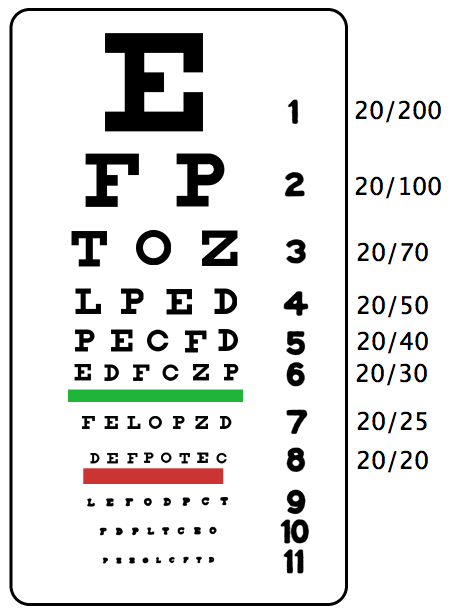
\includegraphics[width=7cm]{figuras/snellen_chart.png}
		}{
			\Fonte{\citeonline{Falkenstein2008}}
		}	
	\end{figure}
	
%jeff
\begin{table}[ht]
	\captionsetup{width=13.5cm}%Deixe da mesma largura que a tabela
	\Caption{\label{tab:categories_of_visual_acuity} Categories of visual acuity}%
	\IBGEtab{}{%
		\begin{tabular}{m{6cm}m{3cm}m{3.2cm}}
			\toprule
			\multirow{2}{*}{Category} & \multicolumn{2}{c}{Presenting distance visual acuity} \\
			& Worse than & Equal to or better than\\
			\midrule \midrule
		    0 Mild or no visual impairment & & 6/18 \\			
			1 Moderate visual impairment & 6/18 & 6/60 \\
			2 Severe visual impairment & 6/60 & 3/60 \\
			3 Blindness & 3/60 & 1/60 \\
        	4 Blindness & 1/60 & Light perception \\
        	5 Blindness & No light perception & No light perception \\
			\bottomrule
		\end{tabular}%
	}{%
	\Fonte{\citeonline{WHO2018ICD}.}}
\end{table}	

According to the report Blindness and Deafness \cite{WHO2018Blindness}, the official descriptions of visual impairment and blindness of \gls{WHO} are:
\begin{quotation}
Visual impairment: Decrease or severe reduction in vision that cannot be corrected with standard glasses or contact lenses and reduces an individual’s ability to function at specific or all tasks.
Blindness: Profound inability to distinguish light from dark, or the total inability to see.
\end{quotation}

Each country has their definition of the term ``legally blind''. The United States of America, Canada, and most European countries define as the best-corrected visual acuity of 6/60 or worse in the better eye; and/or a visual field of 20 degrees or less. In Brazil, the ``legal blindnes'' definition only change in the numbers: visual acuity of 360 or worse and/or visual field of 60 degrees or less \cite{BRASIL1999DECRETO1999}.

We consider this work focused on people who are blind (levels 4 and 5 in Snellen chart), but which also consider people who are visually impaired (levels 1, 2 and 3 in Snellen chart) to have a broader view.

Other factors are also important to understand how the visual perception could influence the user interaction. Many works that evaluate technologies for people who are blind or visually impaired also examine as criteria related to vision impairment the age of blindness onset, the time with impairment \cite{Guerreiro2011} and the etiology of blindness (e.g., retinitis pigmentosa, glaucoma, Leber’s congenital amaurosis, retinopathy of prematurity) \cite{Connors2014} or visual impairment (e.g., glaucoma, age-related macular degeneration (AMD), corneal opacities, diabetic retinopathy, childhood blindness, trachoma, and onchocerciasis) \cite{WHO2018Blindness}.

The damage that prevented the vision could be produced by four sources: \textit{(i)} in transparent structures of the eye, such as cataracts and opacity of the cornea; \textit{(ii)} in the retina, such as macular degeneration and retinitis pigmentosa; \textit{(iii)} in the optic nerve, such as glaucoma or diabetes; and \textit{(iv)} in the brain. Blindness may be congenital or acquired. The damage that impedes vision can be caused at birth, at some event throughout the life of the individual or even in the womb.

\subsection{Assistive technology for people who are blind}
\label{subsec:background-assistive-technology}
Many applications areas have been developed to assist people who are blind or visually impaired. In this context, \citeonline{Manduchi2011} present four areas that have been produced research and technologies. The first one is \textit{mobility}, which provides a person who is blind moves safely, gracefully and comfortable, for example, avoiding obstacles. \textit{Wayfinding} promotes the capacity to know and track one’s position concerning the environment and find a route to a destination, for example, accessing spatial information from a distance. \textit{Printed information access} provides the vast printed information only accessible for sight, for example, read magazines. The last area is \textit{object recognition} that uses recognition algorithms to identify generic objects.

To illustrate these areas, see for instance some examples. Mobility and wayfinding areas are known as Orientation and Mobility (O\&M) \cite{Wiener2010,Welch2016}. In this area, the study \citeonline{Sanchez2014} presents the application Audiopolis (Figure \ref{fig:audiopolis}), a video game for navigating throw a virtual city interacting with audio and haptic interfaces. The Audiopolis also has the goal of improving evolving users' cognitive skills.

 	\begin{figure}[h] 
   	    \captionsetup{width=10cm}%Da mesma largura que a figura
		\Caption{\label{fig:audiopolis} A user playing Audiopolis}
		\UFCfig{}{
			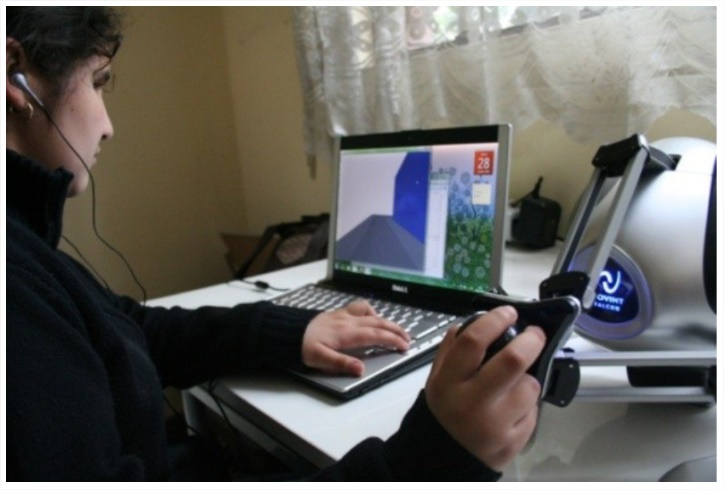
\includegraphics[width=10cm]{figuras/audiopolis.png}
		}{
			\Fonte{\citeonline{Sanchez2014}.}
		}	
	\end{figure}

In printed information access and object recognition areas, with a focus on approaches based on computer vision, the study \citeonline{Maike2016} presents the U-NEXT, an IoT system to perform the tasks of finding and selecting products in a supermarket by using RFID tags and audio feedback as output mode. Figure \ref{fig:U-NEXT} shows a possible scenario of the U-NEXT.

 	\begin{figure}[h] 
   	    \captionsetup{width=9cm}%Da mesma largura que a figura
		\Caption{\label{fig:U-NEXT} U-NEXT smart supermarket scenario}
		\UFCfig{}{
			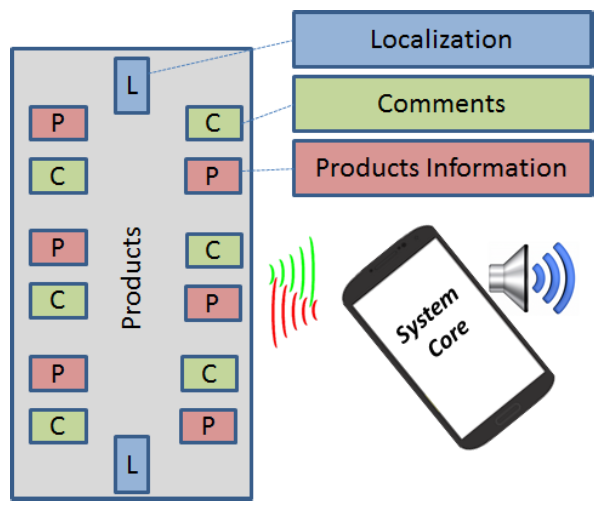
\includegraphics[width=9cm]{figuras/U-NEXT.png}
		}{
			\Fonte{\citeonline{Maike2016}.}
		}	
	\end{figure}

In the face of the large amount and kind of technologies that support the visually impaired and blindness disabilities, \citeonline{Pissaloux2018a} classify the devices that implement these technologies in two sorts: \gls{SSUD} (Sensory SUpplementation Devices) or \gls{SSD} (Sensory Substitution Devices), described as follows.
\begin{quotation}
\textit{\glspl{SSUD} aim to provide to the end user a complementary information which reinforces the user’s personal locomotion capacities and skills. Another sense(s)/modality(ies) are usually put to the contribution. This allows to provide subtle, user expected, cues which ensure that the user’s main attention is on the podo-tactile and auditory cues of the real world, and not on the locomotion cues of the device. Such cues may be exploited during a task execution \cite{Pissaloux2018a}.}

\textit{\glspl{SSD} aim to provide to the end user the information via another (substituting) sense; they offer a new language (new code) which should be learn independently of the initial (natural) role of this sense: a specific stimulus (a code) is associated with each object supposed to be perceived with a new sense \cite{Pissaloux2018a}.}
\end{quotation}

Considering the main objective of this work, we focus only on \gls{SSUD} (Sensory SUpplementation Devices) that includes computers, mobile devices, wearable devices, IoT systems or others according to the purpose of the application. The device \gls{SSD} (Sensory Substitution Devices), out of our scope, includes sensory replacement, haptics as sensory augmentation, bionic eyes, retinal visual prosthesis, cortical implants and others. This definition is important to plan the methodology used and to delimit the focus.

\section{Evidence-Based Software Engineering (\gls{EBSE})}
\label{sec:background-evidence-based}
The use of evidence-based strategies on software engineering has become more and more applied since the 1990s \cite{Shepperd2012}, and it was strongly influenced by clinical practice and the formation of medicine area. Before the research in software engineering is still too much of advocacy research and more scientific approach to software engineering is needed \cite{Wohlin2000}.

The evidence is used to prove the truth of some assertions. According to \citeonline{Shepperd2012}, empirical scientific evidence means that evidence has been obtained from observation (empirical) and in accordance with scientific principles as methods well known and it is documented in a complete and standard way. 

There are many forms for applying an empirical scientific evidence, for example, controlled experiments and quasi-experiments; case studies; surveys; action research and ethnography. Table \ref{tab:evidence_hierarchy} shows the evidence hierarchy considered in \citeonline{Shepperd2012}, helpful to appraising the value of empirical evidence.

\begin{table}[h]
	\captionsetup{width=16cm}%Deixe da mesma largura que a tabela
	\Caption{\label{tab:evidence_hierarchy} Evidence hierarchy}%
	\IBGEtab{}{%
		\begin{tabular}{m{2cm}m{4cm}m{4cm}m{4cm}}
			\toprule
			 & \textbf{Effectiveness} (how well does the intervention work?) & \textbf{Appropriateness} (how suitable is the intervention in the context) & \textbf{Feasibility} (the wider organizational issues of introducing the intervention) \\
			\midrule \midrule
			\textbf{Excellent} & Systematic review; Multi-centre study & Systematic review; Multi-centre study & Systematic review; Multi-centre study \\
			\textbf{Good} & RCT\footnote{RCT means Randomized Controlled Experiments}; Observational study & RCT; Observational study; Interpretive study & RCT; Observational study; Interpretive study \\
			\textbf{Fair} & Uncontrolled trial with dramatic results; Before/after study; Non-randomized controlled trial & Descriptive study; Focus group & Descriptive study; Action research; Before/after study; Focus group \\
			\textbf{Poor} & Descriptive study; Case study; Expert opinion; Poor quality study & Case study; Expert opinion; Poor quality study & Case study; Expert opinion; Poor quality study\\
			\bottomrule
		\end{tabular}%
	}{%
	\Fonte{\citeonline{Shepperd2012}.}%
%	\Nota{esta é uma nota, que diz que os dados são baseados na	regressão linear.}%
%	\Nota[Anotações]{uma anotação adicional, seguida de várias outras.}%
    }
    \end{table}

%%%Figura Excluídda e comentada %%%
\begin{comment}
 	\begin{figure}[h] 
   	    \captionsetup{width=16cm}%Da mesma largura que a figura
		\Caption{\label{fig:evidence_hierarchy} Evidence Hierarchy}
		\UFCfig{}{
			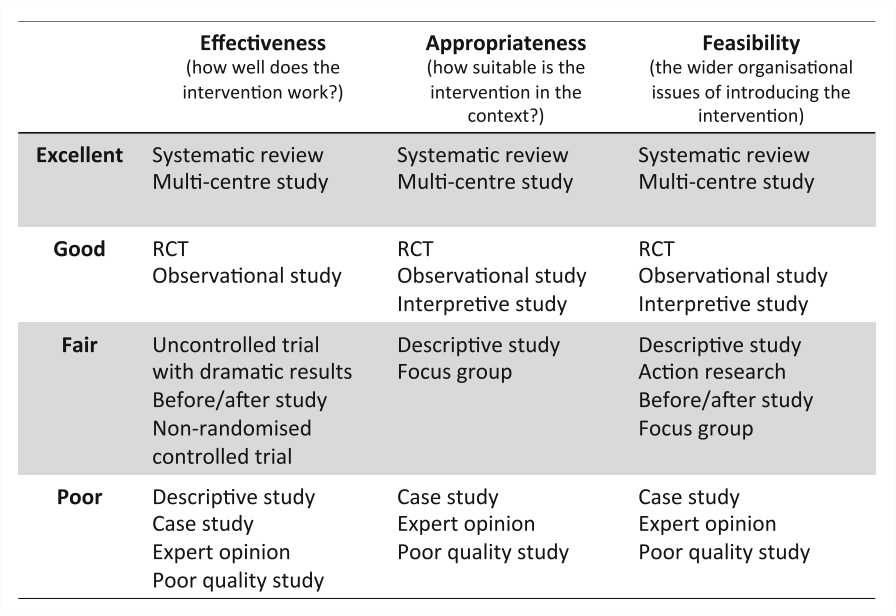
\includegraphics[width=16cm]{figuras/an_evidence_hierarchy_considered.png}
		}{
			\Fonte{\citeonline{Shepperd2012}.}
		}	
	\end{figure}
\end{comment}

\citeonline{Wohlin2000} consider three main empirical strategies in software engineering: \textit{(i)} setting up formal experiments; \textit{(ii)} studying real projects in industry, i.e., performing a case study; and \textit{(iii)} conducting surveys through, for example, interviews.

Considering the purpose of this work for evaluating the impact and effectiveness, we will focus on the experiment as the primary strategy to get evidence. Also, we explore surveys and case studies as empirical methods that have the same purpose. We expect to enable understanding and identification of relationships between different factors, or variables, that affect the use of technology for people who are blind or visually impaired. 

\section{Multimodal Interfaces}
\label{sec:background-multimodal-interfaces}
The perception of humans in their environment occurs through the five senses: vision, hearing, touch, taste, and smell. A mode or modality refers to receiving stimuli from one of these senses \cite{Turk2013}. The unimodal communication is not typical in the information exchange in the human communication. Usually, speech, gestures, facial expressions and others are used at the same time, as well when a person is speaking, he makes gestures to express better their feelings and emotions \cite{Turk2013}.

When a computational system works as multimodal interfaces, it enables the combination of multiple modes or channels of communication between the user and the device in the same interaction \cite{Oviatt2003}. These modes can be used sequentially or simultaneously and, in combination or independently, beyond the traditional input via keyboard and mouse, and monitor output \cite{Neto2008}. The use of multimodal interfaces increase the interaction quality as a result of \textit{(i)} supporting and accommodating the perceptive and communicative capacities of the users; and \textit{(ii)} integrating computational skills in the real world by offering more natural ways of interacting with humans \cite{Dumas2009}. According to \citeonline{Dumas2009} multimodal interfaces are:
Multimodal interfaces process two or more combined user input modes— such as speech, pen, touch, manual gestures, gaze, and head and body movements— in a coordinated manner with multimedia system output. They are a new class of interfaces that aim to recognize naturally occurring forms of human language and behavior, and which incorporate one or more recognition-based technologies (e.g., speech, pen, vision).

Such systems have the potential to function in a more robust and stable way than unimodal recognition systems involving a single interaction technology, such as speech, pen, or vision \cite{Oviatt2003}. \citeonline{Hauptmann1993} concluded that 71\% of the individuals surveyed prefer to use their hands and voice to control objects than a single isolated modality. Some studies seek to understand if the multimodal interaction is capable of facilitating user interaction with a computational system. Other works focus on specific combinations of input and output modes, for example, Interface Web/speech \cite{Neto2008}.

According to \citeonline{Dumas2009}, multimodal systems have the potential to improve Human-Computer Interaction in several ways, as increasing the robustness of systems combining different sources of information; flexible system customization, user-based and context-based; applicability in multi-user systems with mobile interaction; accessibility, since the system presents other alternative forms of interaction; ease of use of small and complex devices allowing more natural interaction in the execution of tasks \cite{InacioJunior2007}.

Inspired by Norman’s action cycle, \citeonline{Dumas2009} illustrates the model of multimodal man-machine communication (Figure \ref{fig:multimodal_man-machine_interaction}) with the major concepts that should be considered for multimodal systems: the fusion of multimodal inputs, and the multimodal fission to generate an adequate message to the user, according to the context of use, preferences and profile.

 	\begin{figure}[h] 
   	    \captionsetup{width=16cm}%Da mesma largura que a figura
		\Caption{\label{fig:multimodal_man-machine_interaction} Multimodal man-machine interaction}
		\UFCfig{}{
			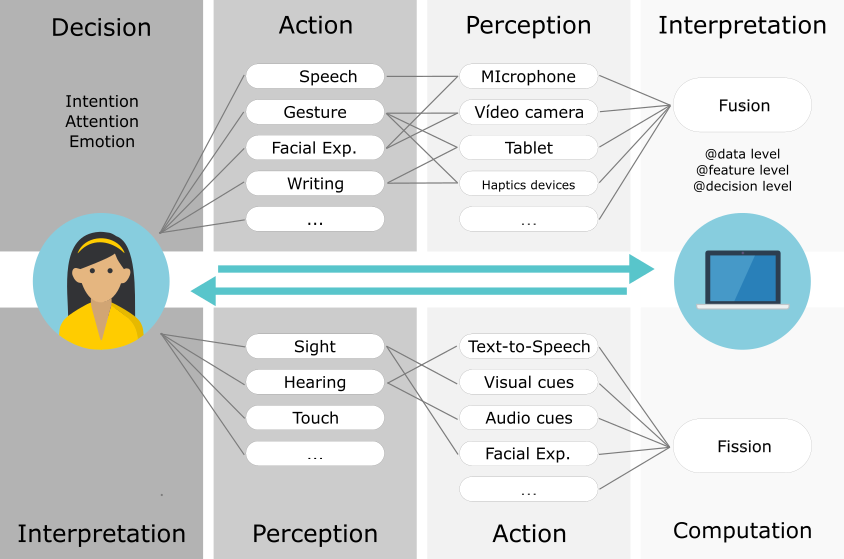
\includegraphics[width=16cm]{figuras/multimodal_man-machine_interaction.png}
		}{
			\Fonte{Adapted from \citeonline{Dumas2009}.}
		}	
	\end{figure}

This interaction between computer and human occurs in four states. On the user's side, the first is the decision state, where the content of the communication message is prepared consciously, intentionally or not, through attention and emotion. The second state is the state of action, where the media are selected, such as voice, gestures or facial expressions. On the computer side, the message is interpreted in the state of perception, where multimodal systems receive information from one or more sensors, at one or multiple levels of expression. In the state of interpretation, the system will attempt to give some meaning to the information received from the state of perception. This is typically the place where the merging of multimodal messages occurs. It is also in this state where the action is taken according to the system's business logic and defined management rule.
        
Depending on the meaning extracted in the interpretation, a response is generated and transmitted, which is where the fission occurs and determines the most relevant modalities for returning the message. This depends on the context of use, for example, within a car, and the user profile, for example, people who are blind.

Furthermore, the theory of processing the interaction requires mental resources at many stages, as shown in Human Information Processing system \cite{Lindsay1977}, described as a model by \cite{wickens2015engineering} as shown in Figure \ref{fig:human_information_processing}. In the Human Information Processing model, the information from the environment is firstly processed by our senses and after that as a Perception. Other elements involved are Attention, Long-term Memory, Working Memory Cognition, Response Selection, Response Execution, and the Feedback.

 	\begin{figure}[h] 
   	    \captionsetup{width=16cm}%Da mesma largura que a figura
		\Caption{\label{fig:human_information_processing} A model of human information processing}
		\UFCfig{}{
			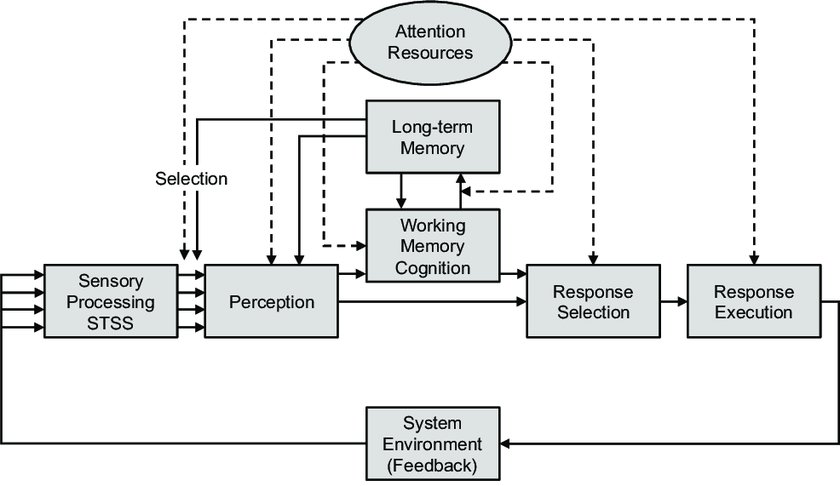
\includegraphics[width=16cm]{figuras/human_information_processing.jpg}
		}{
			\Fonte{\cite{wickens2015engineering}.}
		}	
	\end{figure}

Still related to the multimodal interaction, the proprioception sense could be considered to analyze the interaction on interfaces for people who are blind. The proprioception sense includes the sense of position and movement of our limbs, the senses of muscle force and effort, and the sense of balance \cite{proprioception}. Although it is related to interaction, this dissertation does not study this concept in depth.

Multimodal Interfaces for people who are blind can cover a wider range of users than traditional interfaces, including users of different ages, levels of knowledge, native languages, cognitive styles, impairments and other temporary illnesses or permanent physical disabilities, as well as visual impairment. In this area, blindness and visual impairments present challenges in most stages of human-computer interaction, from input actions, such as touch screen entry and cursor control, to perceiving output, such as interpreting a figure or a diagram \cite{Keates2015}.

While interfaces for the sighted user usually consist of mouse and keyboard as input, interfaces for users who are blind rely principally on auditory information, keyboards, and others haptic devices \cite{Sanchez2014a}. Replacing one mode on multimodal interfaces for another is not a simple solution. Nevertheless, many mobile accessibility solutions for people who are blind commonly replaces the onscreen information only for audio \cite{Guerreiro2011}. This proves that it is necessary to investigate the role of multimodal components in the development and evaluation, as done by \cite{Sanchez2015}. The impact of multimodal interfaces is also reviewed in \cite{Cao2010}, that shows the effect of multimodal interfaces in cognitive and emotional (stress) impact. 

This work aims to provide instruments to verify the real cognitive impact in multimodal interfaces on people who are blind or visually impaired considering the main aspects of multimodal interfaces.

\section{Cognitive Impact Evaluation}
\label{sec:background-cognitive-impact-evaluation}
There are technological aspects to these systems which are investigated from the perspective of how they affect use \cite{Ritter2014}. Cognitive impact concerns the interaction between humans and systems. The field of human-computer interaction has pioneered in the formal study of the cognitive relationship between a person's activities, the artifact of the computer, and the task \cite{Norman1986}. The technologies could enhance human cognitive capabilities. 

\citeonline{Darin2015} literature mapping study shows the cognitive process analyze applications according to a four-dimensional classification (Interface, Interaction, Cognition, and Evaluation). The evaluation dimension includes two main aspects: usability and cognitive impact. 

%\todo[inline]{RETIRADO - This last one assures that an application can develop or enhance any cognitive skills for people with visual disabilities.}

Still on this study, the cognition dimension comprises six skills: mental models, mental maps, spatial structures, Orientation and Mobility (O\&M), problem-solving, and social collaboration. Such approach addresses the main cognitive skills developed and enhanced for impact evaluation purposes. These dimensions could provide directions to define tasks in an experiment to measure the cognitive impact as detection of some obstacles, a useful data for evaluating O\&M \cite{Pissaloux2018a}. 

The study also shows that most papers classified in main cognitive skills are about Mental Map and O\&M. The O\&M skill is a broad concept that is also related to wayfinding and navigation. According to \citeonline{Pissaloux2018a}, ``Human mobility is one of the most important cognitive tasks. Indeed, independent and secure mobility in real physical space has a direct impact on the quality of life, on well-being, and on integration in the numeric society.''

\citeonline{Darin2017} define mobility in a four-dimensional problem: \textit{walking}, \textit{wayfinding} (or orientation), \textit{space awareness} (or space knowledge) and \textit{navigation}. According to this definition, walking is a low conscious cognitive task and involves displacement in the near space. It takes in account obstacle detection and localization. The wayfinding is a set of processes to know one’s current position in space to reach one’s target. The space awareness requires a high consciousness level. It includes forming mental maps, e.g., know the name of the street on a plan. The navigation, the highest-level cognitive task, is a result of the implementation of all listed above functions while traveling.

The impact evaluation of software could use several evidence-based methods. This work focuses on the experiments. To treat the cognitive impact evaluation is necessary to comprehend the experiment design in both cognitive psychology and software engineering areas. The two main theoretical background bibliography used in this work are the books ``Cognitive Psychology'' \cite{Sternberg2011} and ``Experimentation in Software Engineerin'' \cite{Wohlin2000}. In this multidisciplinary context, the next two subsections are dedicated to explain each point of view and highlights the differences. Aside from experiments, the cognitive workload could be measured by an instrument of evaluation, as the questionnaire Nasa-Task Load Index (NASA-TLX) \cite{Hart2006Nasa-TaskLater}, which is a multi-dimensional scale designed to obtain workload estimates from one or more operators while they are performing a task or immediately afterwards.

\subsection{Design experiment in software engineering}
\label{subsec:background-design-experiment-software-engineering}
The experiment process includes several steps: Scoping; Planning; Operation; Analysis and interpretation; Presentation and package \cite{Wohlin2000}. Figure \ref{fig:overview_of_the_experiment_process} presents an overview of the experiment process and artifacts produced. This process provides a high level of control, which uses a formal, rigorous and controlled investigation. Its steps were used to analyze the data of experiments in the methodology proposed (Chapter \ref{chap:metodologia}). Also, the guidelines proposed in this work have the attribute ``when'' that provides in which phase the guidelines are applied.

 	\begin{figure}[h] 
   	    \captionsetup{width=16cm}%Da mesma largura que a figura
		\Caption{\label{fig:overview_of_the_experiment_process} Overview of the experiment process}
		\UFCfig{}{
			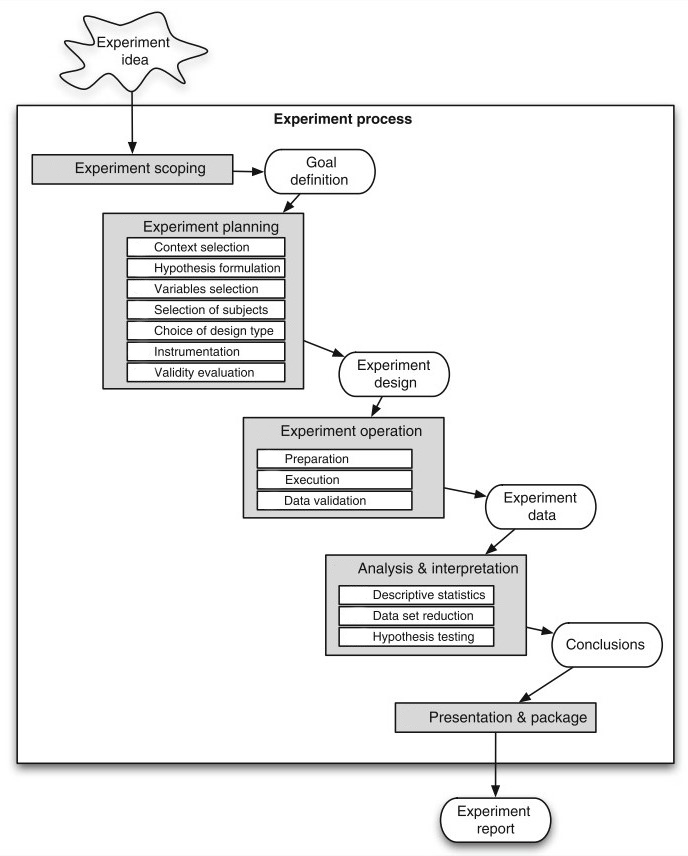
\includegraphics[width=16cm]{figuras/overview_of_the_experiment_process.png}
		}{
			\Fonte{Adapted from \citeonline{Wohlin2000}.}
		}	
	\end{figure}

The main concepts involved in the experiment, shown in Table \ref{tab:the_main_concepts_of_experimental_design}, are used to understand how the cognitive impact is evaluated and to conduct the designing of the guidelines. Figure \ref{fig:variable_relationship_in_the_experiment_process} shows how these concepts are related to the experimental process.

\begin{table}[h]
	\captionsetup{width=16cm}%Deixe da mesma largura que a tabela
	\Caption{\label{tab:the_main_concepts_of_experimental_design} The main concepts of experimental design}%
	\IBGEtab{}{%
		\begin{tabular}{m{2cm}m{13cm}}
			\toprule
			Concepts & Description \\
			\midrule \midrule
			Measure & A mapping from the attribute of an entity to a measurement value. \\
			Instrumentation & The instruments for an experiment are of three types, namely objects, guidelines and measurement instruments. \\
			Dependent Variables & The dependent variables are those we want to see the effect; the independent variables are those controlled and manipulated. \\
			Independent Variables & The independent variables are those controlled and manipulated. \\
			Factors & The independent variables which the experiment changes to verify the effect. Treatment is one value of a factor. \\
			\bottomrule
		\end{tabular}%
	}{%
	\Fonte{\citeonline{Wohlin2000}.}%
%	\Nota{esta é uma nota, que diz que os dados são baseados na	regressão linear.}%
%	\Nota[Anotações]{uma anotação adicional, seguida de várias outras.}%
    }
    \end{table}

 	\begin{figure}[h] 
   	    \captionsetup{width=16cm}%Da mesma largura que a figura
		\Caption{\label{fig:variable_relationship_in_the_experiment_process} Variable relationship in the experiment process}
		\UFCfig{}{
			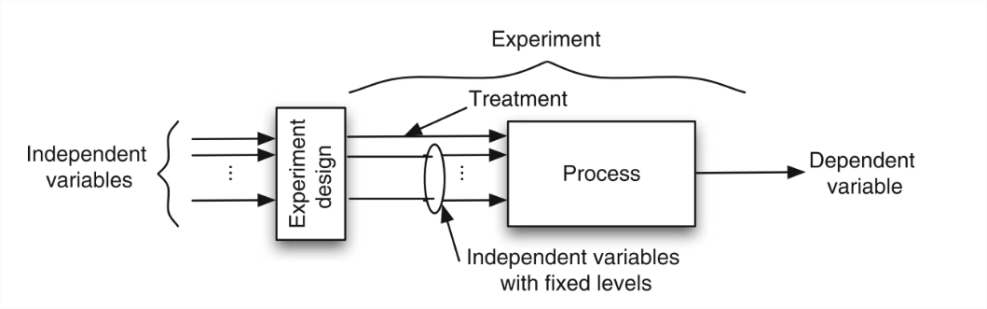
\includegraphics[width=16cm]{figuras/variable_relationship_in_the_experiment_process.png}
		}{
			\Fonte{\citeonline{Wohlin2000}.}
		}	
	\end{figure}

The treatments are measured in the dependent variable, often only one \cite{Wohlin2000}. The variable is mostly not directly measurable, and the experimenter have to measure it via an indirect. Wohlin defines measurement and measure as: ``measurement is the process by which numbers or symbols are assigned to attributes of entities in the real world in such a way as to describe them according to clearly defined rules''. A measure is the number or symbol assigned to an entity by this relationship to characterize an attribute.

As an example of experiment process, we consider the measurements, instrumentation, and variables from the experiment conducted in \citeonline{Connors2014}. In this study, the authors evaluate the navigational performance the of virtual environment called Audio-based Environment Simulator (AbES) that can be explored for the purposes of learning the layout of an unfamiliar, complex indoor environment. The dependent variable evaluated was the navigation performance (Orientation \& Mobility, O\&M).

Some information about the participants is controlled and works as independent variables such as etiology of blindness, age, gender, hand preference, and verbal memory (assessed by using the Wechsler Memory Scale). These variables are controlled and fixed to ensure the correct measurement. The factors in the experiment are the age of blindness onset and the interaction condition with AbES. The factors are randomly distributed into groups: early blind and late blind; and gamers, directed navigators, and control group. The measurements variables used are task success, navigation time, and shortest possible path score.

\subsection{Design experiment in Cognitive Psychology}
\label{subsec:background-design-experiment-cognitive-psychology}
The research methods to in Cognitive Psychology focuses on describing particular cognitive phenomena, such as how people preconceived notions regarding what they may find while gathering the data \cite{Sternberg2011}. To achieve the goal, the research should include more than one method. Among them, the literature present that cognitive psychologists use controlled experiments, psychobiological research, self-reports, case studies, naturalistic observation, and computer simulations and artificial intelligence when studying cognitive phenomena \cite{Sternberg2011}.

Focusing on controlled experiments, the Table \ref{tab:experiment_to_cognitive_phenomena} presents characteristics of controlled experiments to explore cognitive phenomena.

\begin{table}[h]
	\captionsetup{width=16cm}%Deixe da mesma largura que a tabela
	\Caption{\label{tab:experiment_to_cognitive_phenomena} Experiment to cognitive phenomena}%
	\IBGEtab{}{%
		\begin{tabular}{m{3cm}m{12cm}}
			\toprule
			 & Controlled Laboratory Experiments \\
			\midrule \midrule
			Description of method & Obtain samples of performance at a particular time and place. \\ \hline
			Random assignment of subjects & Usually. \\ \hline
			Experimental control of independent variables & Usually. \\ \hline
			Sample representativeness & May be any size. \\ \hline
			Ecological validity & Not unlikely; depends on the task and the context to which it is being applied. \\ \hline
			Information about individual differences & Usually de-emphasized.\\ \hline
			Strengths & Easy to administer, score, and do statistical analyses; High probability of drawing valid causal inferences.\\ \hline
			Weaknesses & Difficulty in generalizing results beyond a specific place, time, and task setting; Discrepancies between behavior in real life and in the laboratory.\\ \hline
			Examples & \citeonline{Karpicke2009} developed a laboratory task in which participants had to learn and recall Swahili-English word pairs. After subjects first recalled the meaning of a word, that pair was either dropped, presented twice more in a studyperiod, or presented twice more in test periods. Subjects took a final recall test one week later.\\ \hline
			\bottomrule
		\end{tabular}%
	}{%
	\Fonte{\citeonline{Sternberg2011}}%
%	\Nota{esta é uma nota, que diz que os dados são baseados na	regressão linear.}%
%	\Nota[Anotações]{uma anotação adicional, seguida de várias outras.}%
    }
    \end{table}

Regarding the experiment concepts, the variables of the experiment are \textit{(i)} independent variables, that are individually manipulated, or carefully regulated, by the experimenter; or \textit{(ii)} dependent variables, that are outcome responses, the values of which depend on how one or more independent variables influence or affect the participants in the experiment \cite{Sternberg2011}. This literature also presents the concepts of \textit{(iii)} irrelevant variables, which affect the outcomes (dependent variable) when manipulated; \textit{(iv)} control variables, which are held constant; and \textit{(v)} confounding variables, which affect the dependent variables without be controlled or manipulated and should be avoided. 

Independent and dependent variables must be chosen with great care, because what is learned from an experiment will depend almost exclusively on the variables one chooses to isolate from the often complex behavior one is observing \cite{Sternberg2011}. The authors suggest two dependent variables that are used in cognitive-psychological research: percent correct (or its additive inverse, error rate) and reaction time. These measures are popular because they can tell the investigator, respectively, the accuracy and speed of mental processing \cite{Sternberg2011}. 

Among the myriad possibilities for independent variables are characteristics of the situation, of the task, or of the participants \cite{Sternberg2011}. For example, characteristics of the situation may involve the presence versus the absence of particular stimuli or hints during a problem-solving task, as virtual versus real navigation \cite{Lahav2008b}. Characteristics of the task may involve reading versus listening to a series of words and then responding to comprehension questions. Characteristics of the participants may include age differences, differences in educational status, or differences based on test scores. Characteristics of the participant are not easily manipulated experimentally due to the ethical regulation.